\documentclass[output=paper%,colorlinks,citecolor=brown,
% hidelinks,
% showindex
]{langsci/langscibook}


\author{Adam Jatowt\affiliation{University of Innsbruck} and
Nina Tahmasebi\affiliation{University of Gothenburg} and
Lars Borin\affiliation{University of Gothenburg}} 


\title[Computational approaches: Visualization systems and novel applications]
      {Computational approaches to lexical semantic change: Visualization systems and novel applications}

\abstract{The purpose of this chapter is to survey visualization and user interface solutions for understanding lexical semantic change as well as to survey a number of applications of techniques developed in computational analysis of lexical semantic change. We first overview approaches aiming to develop systems that support understanding semantic change in an interactive and visual way. It is generally accepted that computational techniques developed for analyzing and uncovering semantic change are beneficial to linguists, historians, sociologists, and practitioners in numerous related fields, especially within the humanities. However, quite a few non-professional users are equally interested in the histories of words. Developing interactive, visual, engaging, and easy-to-understand systems can help them to acquire relevant knowledge. 

Second, we believe that other fields could benefit from the research outcomes of computational approaches to lexical semantic change. In general, properly representing the meaning of terms used in the past should be important for a range of natural language processing, information retrieval and other tasks that operate on old texts. In the latter part of the chapter, we then focus on current and potential applications related to computer and information science with the underlying question: ``How can modeling semantic change benefit wider downstream applications in these disciplines?''
}

\begin{document}
\maketitle

\section{Visualization systems supporting manual analysis}
It is already evident that computational approaches greatly speed up the research and the resulting discoveries related to semantic change and lexical replacement. The applications of this research progress still remain to be seen, both inside and outside the academic realm.
Providing effective methods for detecting changes, their characteristics, timing, and causal factors are all important for our understanding of languages and their evolution. Computational methods support the acquisition of such knowledge and the formation and validation of various kinds of hypotheses. However, other uses of the  technology outside the academic field are less discussed. 
Word meaning change is not only interesting to professionals (e.g., linguists, historians, or librarians) but also to the wider public. For example, many books discussing the origins and evolution of word meaning have been published aiming at a wider readership, suggesting significant interest by average users in the histories of words. 
We think that computational approaches and especially online interactive systems are important to help to further disseminate knowledge about  etymology.

\begin{sloppypar}
Visual analytics have been increasingly applied in  historical linguistics \citep{schatzle:hal-02914284} by combining automated algorithms with interactive visual components to let us perform effective investigations through data manipulation and presentation. In this context, several online visualization systems and demonstrations supporting manual analysis have been proposed to complement the research methods developed for detecting diachronic conceptual change. They allow for verification of the results obtained from automatic methods or provide novel means for supporting manual determination of diachronic conceptual change and its characteristics. In these systems the level of interactivity and user freedom in querying the data, as well as the provision of features enabling multidimensional analysis play crucial roles. Evaluation of these systems focuses on usability criteria and their user interfaces. Visualization systems tend to be attractive as they provide either a complement to automatic analysis or serve as the main tool for analysis, and not only for professionals and scientists. Many of them are also particularly suited to lay users, especially if the systems are intuitive and highly usable. Below, we discuss representative  systems designed for learning about semantic change and we highlight several new directions based on their analysis. Due to copyright restrictions, we can only shown the screenshots of few, selected examples.
\end{sloppypar}

\subsection{Description- and frequency-based approaches}
Starting with a simple example, the enhancement of definitions generated by the Google word search engine for ``definition queries'' is an effective way to disseminate basic information on words' origins and patterns of  popularity over time. When given an input word, a standard definition can be complemented by an additional click with a brief textual description of the word's origin as well as its frequency plot over time (see Figure~\ref{fig:google-snapshot} for example). This service provides historical context for word definitions that can support better understanding of queried words and also trigger user interest in word histories by appending complementary basic knowledge about the temporal evolution of word meaning. Although users can see the change in the frequency of a word over time and read brief information on the word's origin, they still essentially have to guess about the word's meaning change over the entire span of time. Nevertheless, this application is worth mentioning because, thanks to the popularity of Google search services, information on word change (albeit rather superficial) can be widely disseminated to the public through this service.

\begin{figure}
	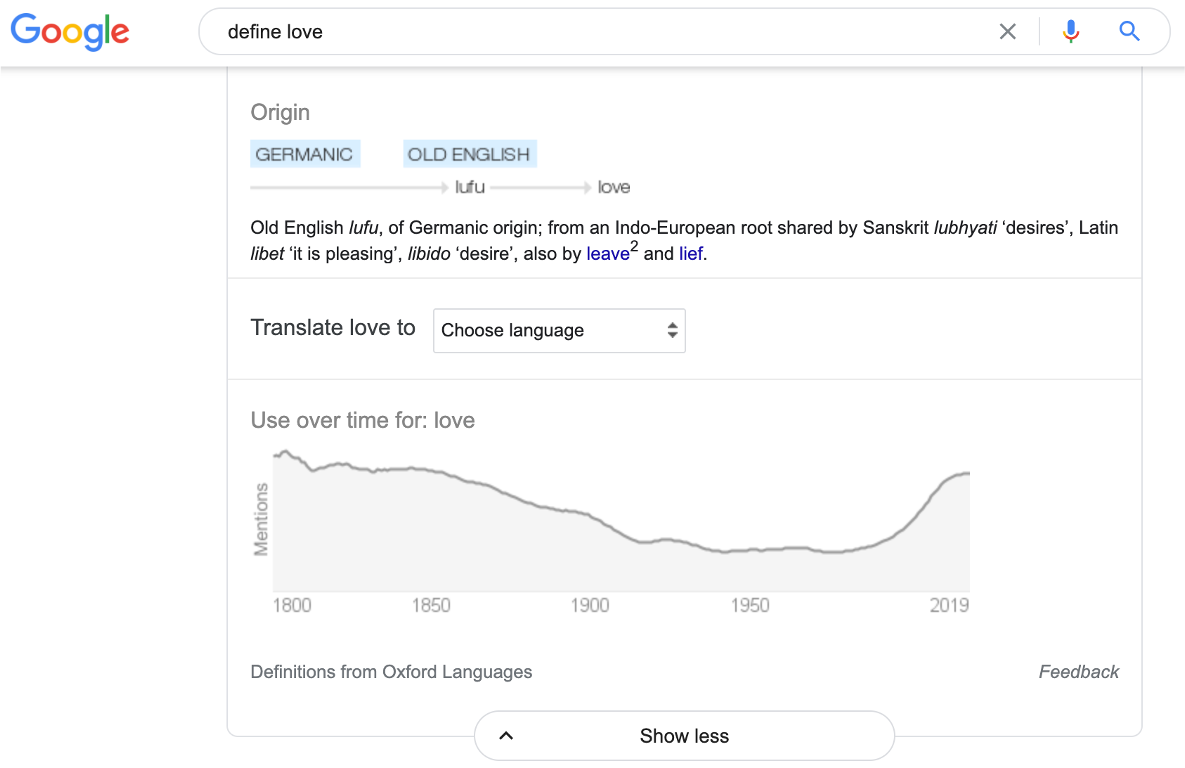
\includegraphics[width=\textwidth]{figures/JATOWT_google_snapshot.png}
        \caption{Snapshot of an example output from Google search engine for the query \texttt{define love} where simple information on the origin and popularity of word \textit{love} over time is given (image captured on 24-01-2021).}
	\label{fig:google-snapshot}
\end{figure}


The \emph{Online Etymology Dictionary}\footnote{\url{https://www.etymonline.com/}} is an easy-to-use system that draws on the etymology of numerous words compiled from several dictionaries. The service returns a short etymological description of an input word with dates indicating the earliest year for which there is a surviving written record of its use. 

The \emph{Google Books Ngram Viewer}\footnote{\url{https://books.google.com/ngrams}} \cite{michel2011quantitative} -- another notable contribution from the search engine company -- is a powerful online application for observing and analyzing the frequency of words or Ngrams over time. It is based on the Google Books Ngrams datasets. The service has frequently been used for digital humanities research and the like \citep[e.g.][]{michel2011quantitative,acerbi-etal-2013,bentley-etal-2014,pechenick-etal-2015,iliev-etal-2016}. The temporal frequency plots of several words or Ngrams can be contrasted with each other. Users can choose a wildcard search (by putting * in place of a word in a given phrase to obtain the top ten substitutions) or do a case-insensitive search. Analysis based on parts of speech (POS) tags is possible (e.g., plotting frequencies of \emph{tackle} as either a verb or as a noun). It is also possible to plot the frequency based on five composition operators (e.g., summing or subtracting the frequencies of several expressions). Inflection-oriented search can be done (e.g., searching with \texttt{\mbox{book\_INF} a hotel} returns results for \emph{book, booked, books}, and \emph{booking a hotel}). The Ngram viewer allows the identification of words at the start or end of sentences to be plotted. 
It provides dependency relations using the => operator. For instance, to understand how often \emph{tasty} was used to modify the word \emph{dessert} one would input (\texttt{tasty} => \texttt{dessert}). This search combines frequencies of all instances in which the word \emph{tasty} modifies \emph{dessert}, including \emph{tasty frozen dessert}, and \emph{tasty yet expensive dessert}. Dependencies can be further combined with wildcards (e.g., \texttt{drink => *\_NOUN} to track frequencies of expressions containing different kinds of beverages as nouns). 
Nevertheless, because the viewer is mainly based on the frequency signals of words (i.e., probabilities of seeing a given Ngram or a set or composite of Ngrams in a given year), it does not provide a direct means for portraying exactly how a term was used in the past or when its meaning transitions occurred. The viewer is thus best suited to culturomics or cultural text mining studies and is similar to other tools available for general purpose interactive exploration of diachronic corpora \citep[e.g.][]{michel2011quantitative,odijk2012time,eijnatten2014using,jatowt2016historycomparator}. Despite this limitation, this application is worth mentioning because it uses extremely large datasets coupled with basic manipulation capabilities,  even though it does not explicitly support  analysis of semantic change.

The online interfaces of several diachronic corpora created by Mark Davies at Brigham Young University\footnote{\url{https://corpus.byu.edu/}} provide effective options for users. Users can perform simple analyses without the need to write any code. For example, they can generate frequency plots over time, examples of keywords in context (KWIC) at different time points, and listings of collocates. However, the amount and level of detail  of the displayed data make it rather difficult to draw broader conclusions about the semantics of words from a longitudinal perspective.

\citet{hilpert2008assessing} apply a variant of hierarchical clustering called vari\-abil\-ity-based neighbor clustering. The idea is to cluster adjacent time units (hence the name ``neighbor clustering'') if the frequency of a target term does not change much. The resulting dendrogram allows for visual identification of time points of large frequency change, which may indicate increased possibility of diachronic sense shifts (e.g., due to sudden triggers like large events). No context is used for a target word because the method relies only on the the frequency information of a query word, which limits the applicability of this approach in representing diachronic conceptual change of words.

\citet{odijk2012time} demonstrate an interactive environment that visualizes information on the volumes and correlations of words and documents across time. Similar to \citet{michel2011quantitative}, their focus is more on understanding historical and social aspects than on shifts in word meaning. 

\subsection{Context-based semantic approaches}
\citet{rohrdantz2011towards} use latent Direchlet application (LDA) to represent the different senses of words and track their intensity of change over time. Twenty-five words before and twenty-five words after the target word are used as the context of the term, following the suggestion given by \citet{schutze1998} for automatic sense discrimination. This approach allows one to notice various kinds of semantic change in words, such as the broadening or narrowing of senses and the first occurrences of senses, especially as all the topics are shown over time in a single view. According to \citet{rohrdantz2011towards}, their interactive visualization approach provides the possibility of detecting key patterns at a glance, while at the same time observing the details of the data by zooming in on the occurrences of particular words in their contexts. Additionally, the results of the pairwise comparisons of word senses with respect to their shared contexts are also displayed. The authors, however, restrict their system to only a short time period, demonstrating results on the New York Times Annotated corpus, which spans roughly two decades. 

\citet{heylen2012looking} propose using a multidimensional scaling \citep{cox2008multidimensional} technique with a window length of 4 words before and after the target word and pointwise mutual information for weighting context terms. 
\citet{heylen2012looking} took this approach because they had observed that earlier automatic approaches which use distributional models use them in an indirect, black-box fashion, failing to indicate particular semantic properties and relations that play key roles. Motion charts from the Google Chart tools are then used to visualize occurrences of nouns in a 2D representation of their semantic distances. Hovering a mouse pointer over the bubbles denoting nouns shows the text in which each noun occurs so that users can interpret the precise meaning of the occurrence of the noun. In their case study, the authors focus on Dutch words extracted from Dutch newspaper articles published between 1999 and 2005, which were organized in 218 synsets containing 476 nouns in total. Although they do not use the motion feature of the charts, the authors admit that it should be possible to track the centroid of the tokens of a target word over time in the semantic space, and also show the dispersion of the tokens around the centroid.

\citet{hilpert2015meaning} use animations in the form of animated scatterplots to portray change in patterns over time using the metaphor of a petri dish. The authors focused on a single pattern, ``many a [noun]'' as a case study. Spots on the graphs represent nouns involved in the same pattern, and are plotted next to each other if they have high similarity. The size of the spot is linked to the frequency of a noun or noun type in a particular time unit. During the animation, the changes in the size and distances of spots provide knowledge of different uses of the pattern over time.

\begin{sloppypar}
Dimensionality reduction techniques such as principal components analysis (PCA), latent semantic analysis (LSA) or the popular t-distributed stochastic neighbor embedding (t-SNE, \citealt{maaten2008visualizing})\footnote{\url{https://lvdmaaten.github.io/tsne/}} have been frequently used to plot ``trajectories'' of word meaning over time in vector spaces using 2D plots. By showing points that represent the meaning of the same words at different years or decades on the same 2D plot \citep[see, e.g.,][]{hamilton-etal-2016-cultural,kulkarni2015statistically}, and optionally connecting them with arrows, a single static view can show how the words changed their meaning over time, by simply following their ``trajectories''. Typically some background reference terms are added along these ``trajectories'' to ground and explain the meaning.
\end{sloppypar}


\citet{martinez2016design} introduce a system called \emph{ShiCo} for visualizing shifting concepts of Dutch words over time. It measures change in words used to refer to concepts based on a model previously introduced by \citet{kenter2015ad}. This model requires a series of semantic spaces that are constructed by training word embeddings (e.g., word2vec) for different units of time (typically, each unit spans 10 years). It is based on two steps, generation and
aggregation. The generation step works in an iterative fashion. An initial seed set is selected that typically consists of a small number of user-provided terms. Then, words most semantically similar to the seed set are found based on similarity values between word embeddings. A semantic graph is constructed from these terms, and the central terms are extracted using graph centrality measures. Next, the central terms are used as the seed set for the next iteration of the generation step. In the
aggregation step, the lists of words produced in the generation step are aggregated to generate the final word lists to be presented to the user.
The visualization by \citet{martinez2016design} is composed of two kinds of complementary graphs: a stream graph and a series of network graphs. The former shows color-coded streams for each term; the stream sizes represent the relative importance of the term in a period. This importance is measured either as  a term count in each time unit or as a sum of the similarities of the term to the seed terms. The network graphs for each time unit display the relations between terms in the time unit. 

\citet{xu2017temporal} use term clouds and a heatmap to visualize semantic shifts of target words by utilizing sequentially trained embedding vectors with initialization based on previous time periods, as proposed by \citet{kim-etal-2014-temporal}. They use \textit{The New York Times} and \textit{National Geographic Magazine} articles for the underlying datasets, which span about 110 years. Following \citet{martinez2016design}, a temporal semantic similarity word cloud is used to show terms most similar to a target query for a given time unit. As in standard term clouds, the font size of the terms is linked to their similarity to the query word. Heatmap views let users see the similarity values of the terms most similar to the target term in each year, using colors. The y-axis of the heatmap is a list of words and the x-axis is a list of temporal periods such that for each given word (each row) one can understand the pattern of the change in the similarity of this term to the target term (also called anchor term). The results from the \textit{The New York Times} and \textit{National Geographic Magazine} are then contrasted with each other. 

\begin{sloppypar}
\citet{jatowt:2014:fas:2740769.2740809} describe an analytical framework that incorporates different types of similarity plotting. The plots include across-time self-similarity, a decade-to-decade similarity heatmap, across-time sentiment analysis, diachronic comparative word analysis, and key context term listing. They use both the Google Books Ngrams and COHA datasets. The signals from the different views (e.g. frequency analysis, semantic analysis, and sentiment analysis) can be combined to allow for multi-evidence-based reasoning on diachronic conceptual change. Two different word representations are used: a simple bag-of-words, and a distance-aware bag-of-words, where the distance used is the relative position of a context term to the target term. For simplicity, the sentiment values of context terms are assumed to remain stable over time when computing the change of the sentiment of the target term's context. 
\end{sloppypar}

Their work resulted in the development of an online interactive system for diachronic conceptual change analysis \citep{jatowt2018every} (see Figures~\ref{fig:jatowt0}, \ref{fig:jatowt2} and \ref{fig:jatowt3}).\footnote{\url{http://www.okayama.silk.jp/WordEvolution/}} The system enables detailed analysis of diachronic conceptual change from different viewpoints, such as word's context comparison across-time, temporal term cloud, and temporal term tree generation. It can also perform contrastive analysis of word pairs (see Figure~\ref{fig:jatowt0}) of larger groups of words such as synonyms. The results can be generated using both the Google Books Ngrams and COHA datasets. Pearson correlation, cosine similarity, and Jaccard similarity can be used as similarity measures of word representations from different time points. \citet{jatowt2018every} recommend that diachronic conceptual change over time should be contrasted with term frequency plots \citep[as also suggested by][]{kim-etal-2014-temporal}, since together both provide a more informed view on how often and in what sense a term was used in the past. Any conclusions drawn from semantic change plots should be treated with caution when the frequency plot of a target term shows a low utilization rate. To better visualize the word change in relation to the average change of other words, the degree of the target word's change over time is also displayed with reference to the average change of words in the same frequency bin as the target word.

The system has another novel feature that allows the change in individual context terms over time to be investigated in the form of a \emph{time-enhanced term cloud} (see Figure~\ref{fig:jatowt2}) and \emph{time-enhanced term tree} (see Figure~\ref{fig:jatowt3}). Finally, the framework provides a unique functionality to track the semantic shifts of entire concepts represented as word sets, for example, the concept of a vehicle represented by words like \emph{auto}, \emph{automobile}, \emph{car}, \emph{truck}, and so on. 

\begin{figure}
	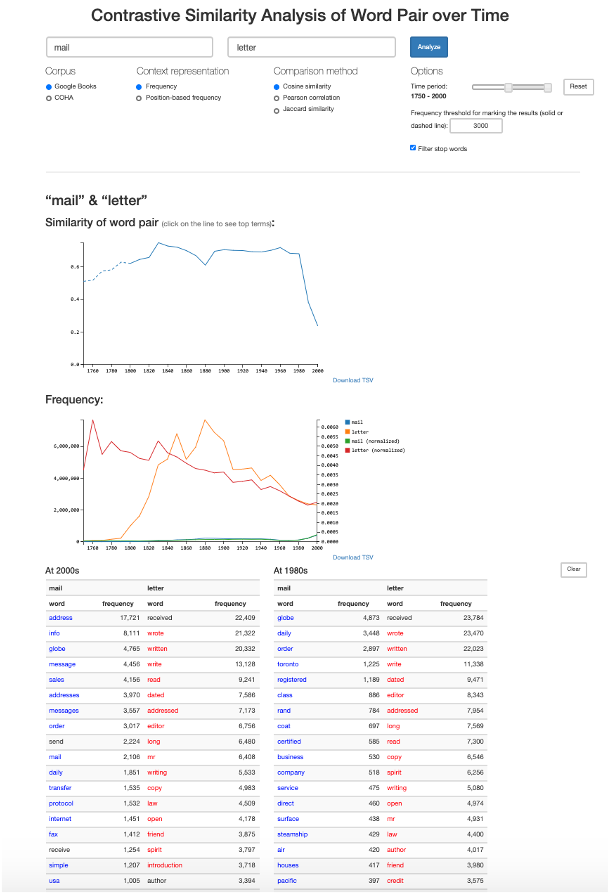
\includegraphics[width=.915\textwidth]{figures/JATOWT_jatowt0.png}
        \caption{Snapshot of an example output from the diachronic conceptual change analysis system for comparing the words \textit{mail} and \textit{letter} that displays their similarity plot over time, frequency plots and the contrasted lists of top-frequent context term at 1980s and 2000s (image captured on 24-01-2021).\label{fig:jatowt0}}
\end{figure}

\begin{figure}
	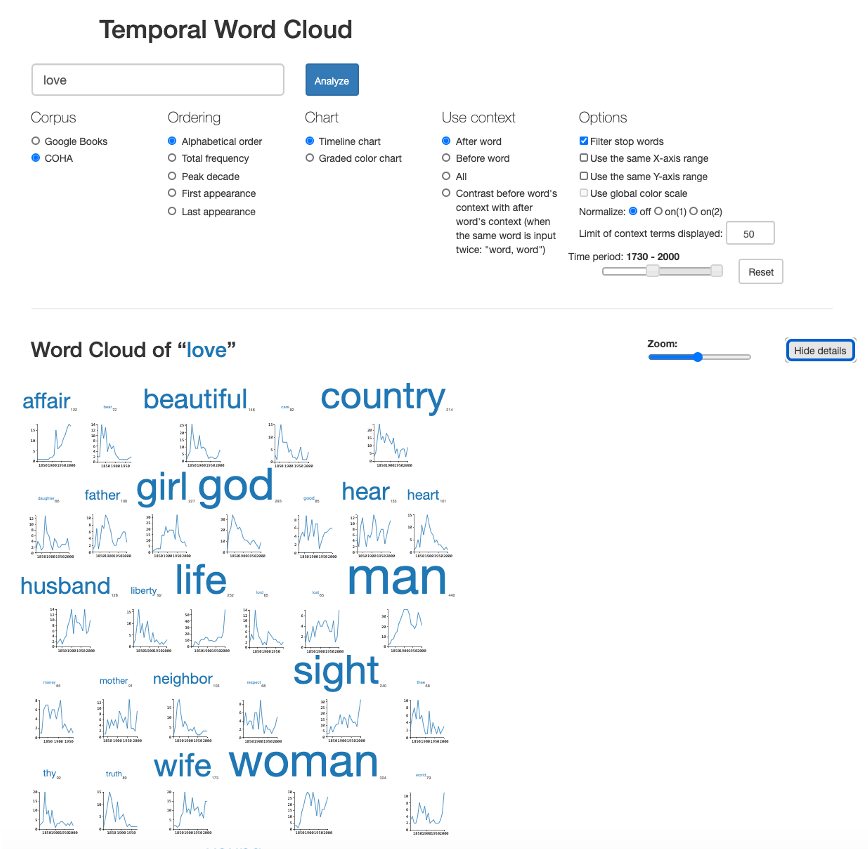
\includegraphics[width=\textwidth]{figures/JATOWT_jatowt2.png}
        \caption{Snapshot of an example output from the diachronic conceptual change analysis system for the word \textit{love} which shows a part of temporal term cloud of context words for an input word \textit{love} (image captured on 24-01-2021).\label{fig:jatowt2}}
\end{figure}

\begin{figure}
	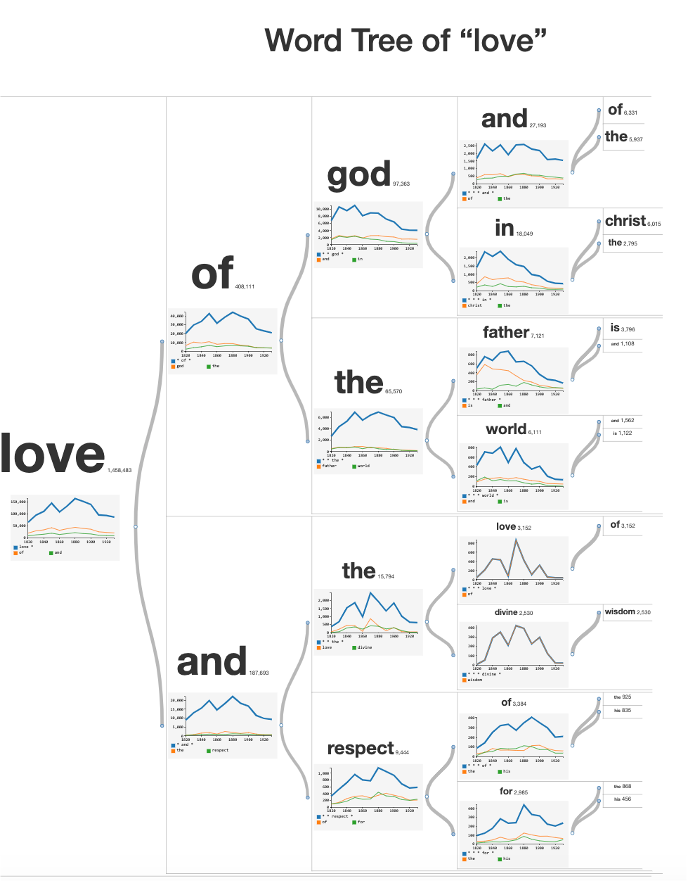
\includegraphics[width=.75\textwidth]{figures/JATOWT_jatowt3.png}
        \caption{Snapshot of an example output from the diachronic conceptual change analysis system which shows a part of temporal term tree for an input word \textit{love} (image captured on 24-01-2021).\label{fig:jatowt3}}
\end{figure}

\citet{jeseme} proposed JeSemE, the Jena Semantic Explorer,\footnote{\url{http://jeseme.org/}} which is an interactive website for visually exploring temporal information on word meanings and lexical emotions on the basis of five large diachronic text corpora in English and German, including COHA and Google Books English fiction. A unique feature of this system is the provision of predicted emotion values of words over time based on the valence-arousal-dominance (VAD) scheme of \cite{bradley1994measuring}. It also shows similar words and specific contexts of a query word. Figure~\ref{fig:jeseme1} and \ref{fig:jeseme2} show example outputs.

\begin{figure}
	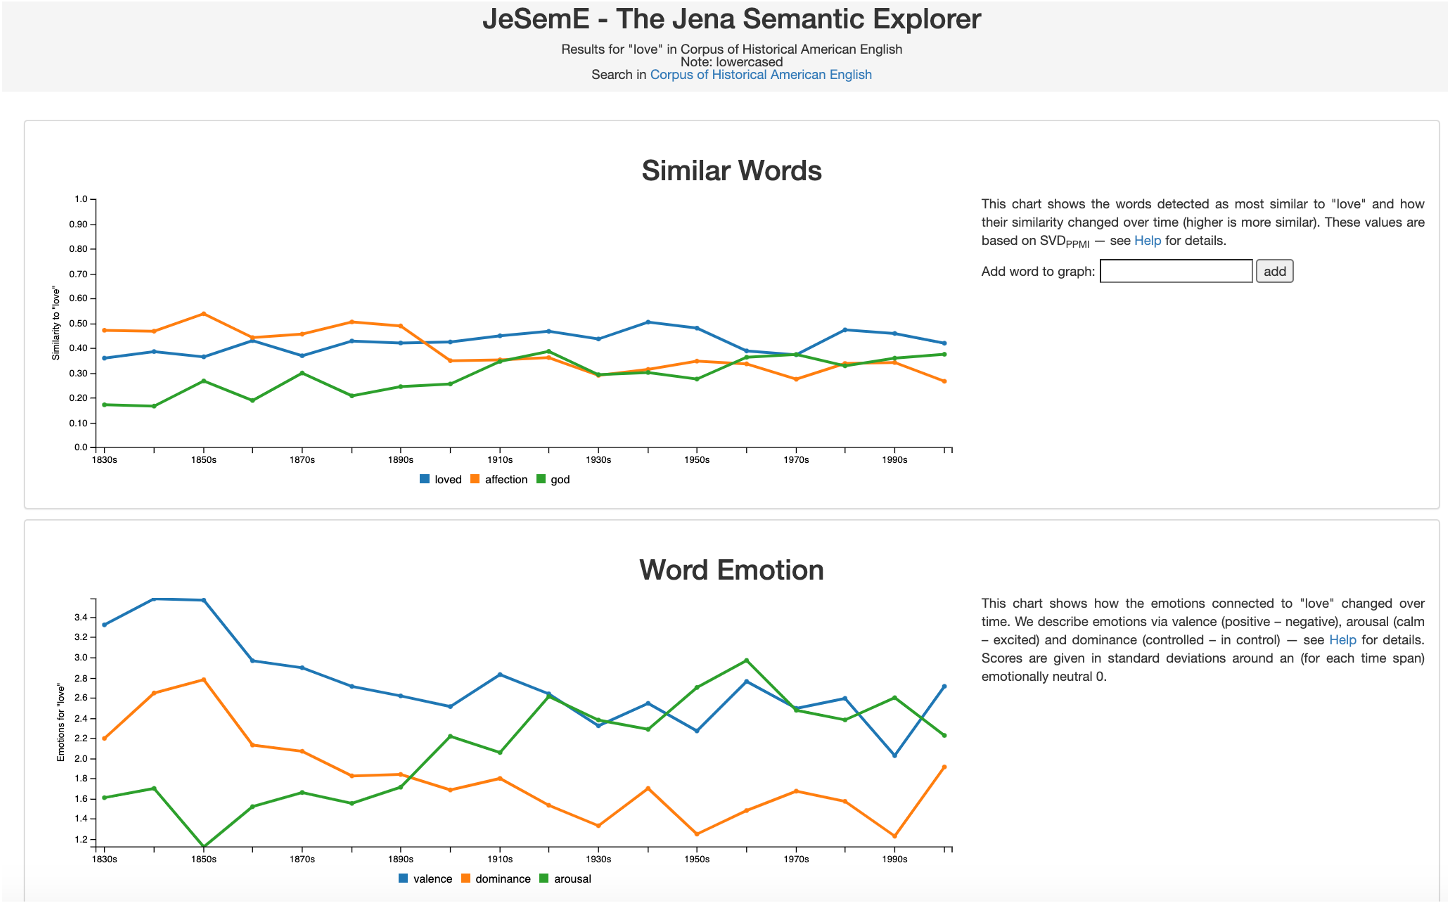
\includegraphics[width=.9\textwidth]{figures/JATOWT_Jeseme1.png}
        \caption{Snapshot of an example output from JeSemE for word \textit{love} which shows the similarity of similar words to the input word and associated emotions over time (image captured on 24-01-2021).\label{fig:jeseme1}}
\end{figure}

\begin{figure}
	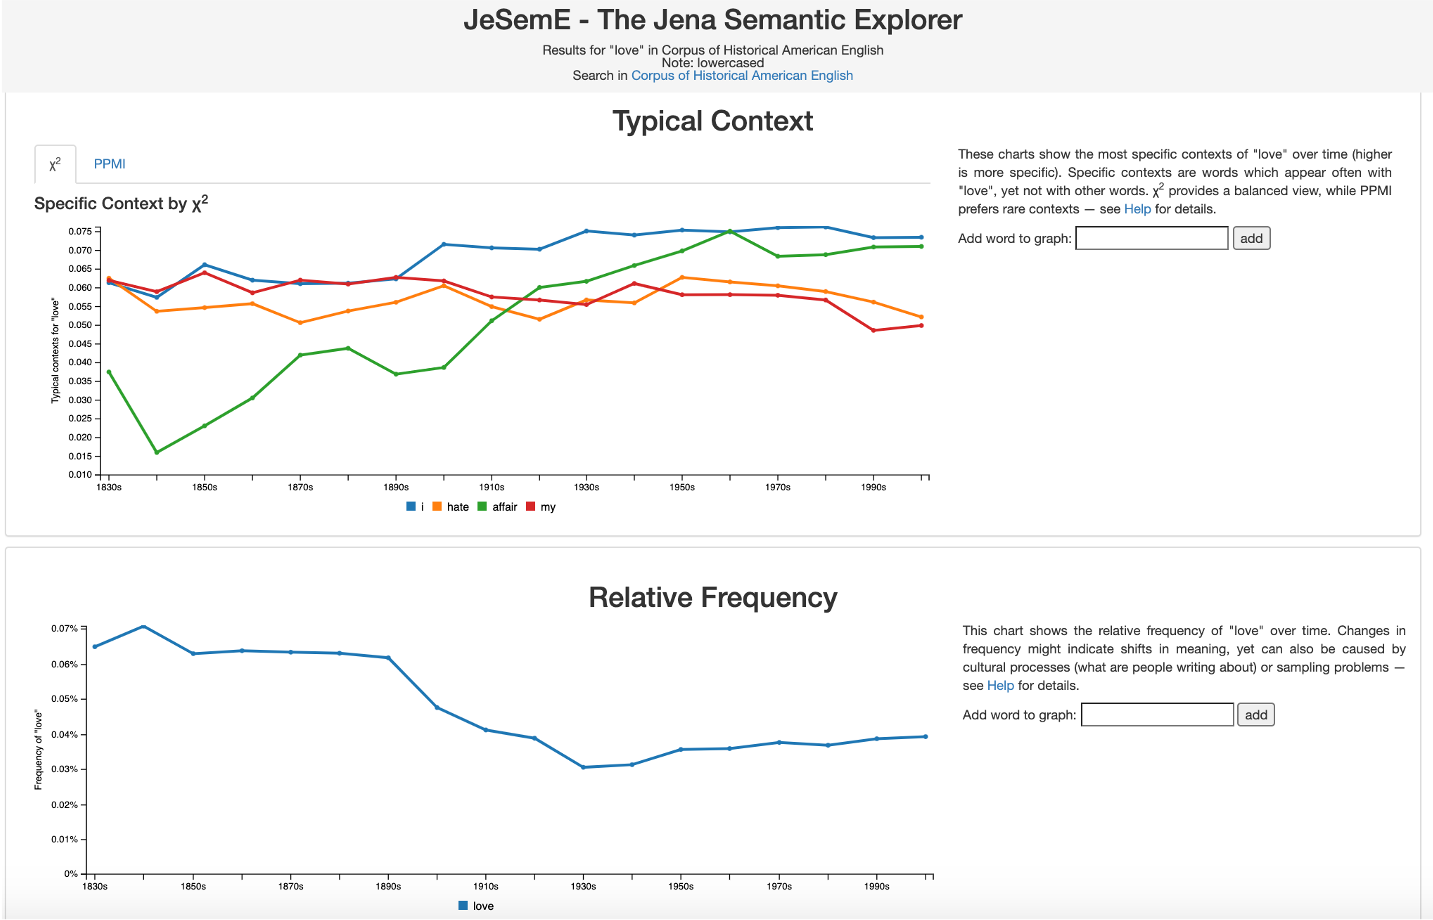
\includegraphics[width=.9\textwidth]{figures/JATOWT_Jeseme2.png}
        \caption{Snapshot of an example output from JeSemE for word \textit{love}  which shows specific context words and relative word frequency over time (image captured on 24-01-2021).\label{fig:jeseme2}}
\end{figure}

\subsection{Dictionary-based approaches}
\citet{theron2015diachronic} demonstrate an interactive visual tool for advanced analysis of the data in Spanish historical dictionaries. Their approach is unique as they utilize different editions of Spanish language dictionaries over time: the 1780, 1817, 1884, 1925, 1992 and 2001 editions provided by the Royal Spanish Academy. 
In this method the dictionary editions are arranged in a matrix in columns (right to left in  chronological order), while the meanings of a word are placed on the rows (top to bottom in ascending order). Lines are drawn to connect  related meanings across time, with the connection computed using  NIST or BLEU metrics \citep{zhang2004interpreting}, which are frequently utilized in evaluating machine translation or summarization accuracy. Starting from the most recent dictionary, a particular meaning is connected to its closest meaning in the previous dictionary; if there is nothing that satisfies the predefined similarity threshold, then the procedure is repeated with the older dictionary. Connecting lines can have branches in cases of bifurcation or merging of meanings. \citet{theron2015diachronic} call the resulting diagrams \emph{diachronlex diagrams}. The diagrams can be further improved by collapsing nearby lines with similar temporal patterns or by simplifying branches. Furthermore, users with editing rights can annotate meanings or change their associations.


\subsection{Systems for analyzing lexical replacement}
\citet{mazeika2011entity} focus on semantically similar entities from different time periods to provide visual support in analyzing lexical replacement, particularly for entities. They extracted named entities from the Yet Another Great Anthology (YAGO) database to provide a visual analytics tool to analyze the evolution of named entities in the New York Times Annotated Corpus. Name changes are not tracked, but the tool offers a visualization of the evolution of an entity in  relation to other entities. 

Investigation of lexical replacement and temporal analogy are also  possible in the aspect-based temporal analog retrieval (ATAR) system \citep{zhangwsdm} which uses perceptrons to compute transformations between present and past vector spaces trained on the present and past participles, respectively. For a user query (e.g., \emph{Euro}) and its defining aspect or sense (e.g., \emph{currency}) a list of analogical terms is produced based on the analysis of its past document collection, together with an extracted representative sentence for each output term (see Figure~\ref{fig:wsdm}). The sentence provides a typical context in which an analogous word was used in the past, using the output style dubbed KWECT (keyword in exemplar context at time), similar to the traditional KWIC (keyword in context) style. 

\begin{figure}
	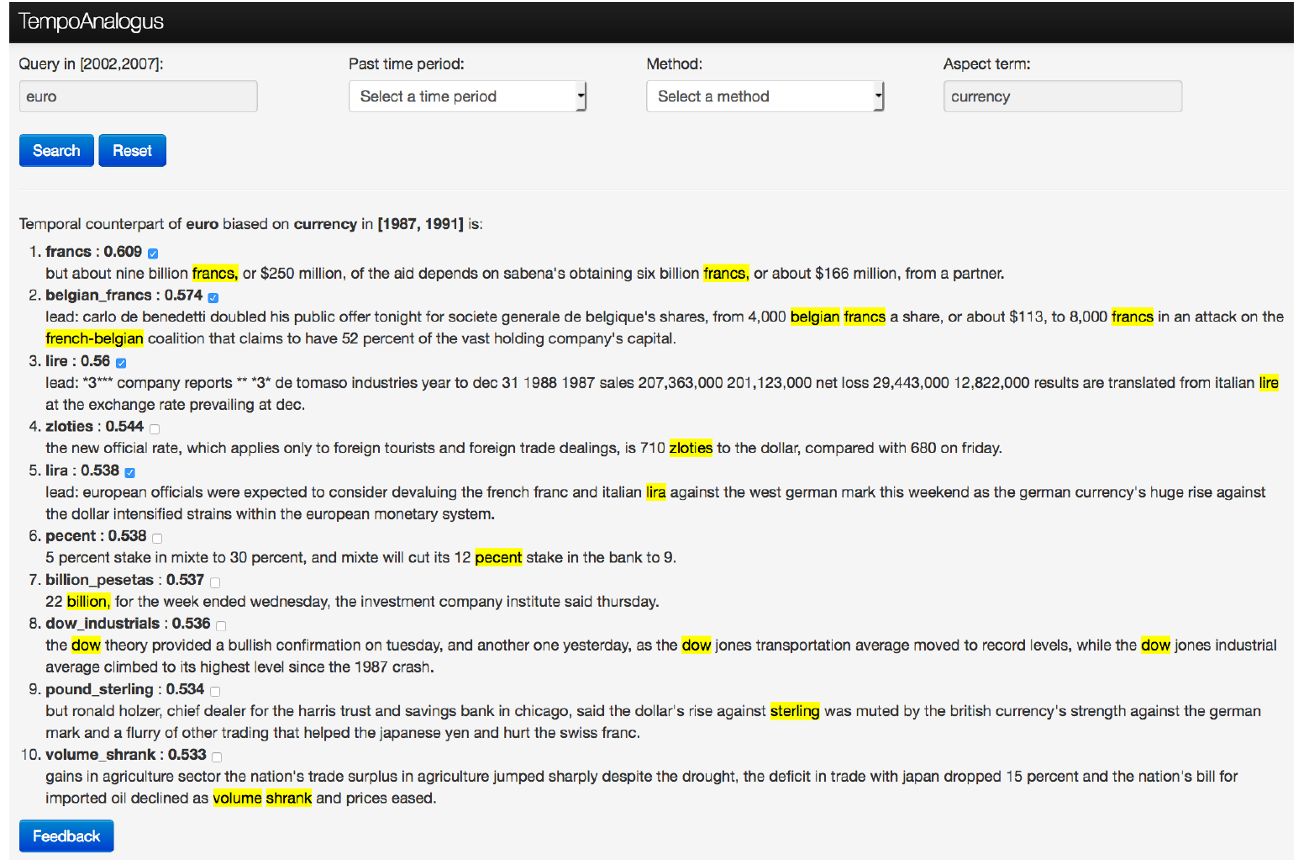
\includegraphics[width=\textwidth]{figures/JATOWT_WSDM.png}
    \caption{Snapshot of an example output from aspect-based temporal analog retrieval system (ATAR) for the query word \emph{Euro} under the aspect of currency (image captured on 24-01-2021).\label{fig:wsdm}}
\end{figure}


\subsection{Summary and observations}
Visualization and analysis of diachronic conceptual change belong to an emerging and powerful research field of interactive visualization for computational linguistics \citep{collins2008interactive}. Its purpose is to let users understand models of language and their abstract representations, and to visually uncover patterns in language. In view of the inherent complexity of tracking word senses and understanding their shifts over time, we expect an increase in the availability and popularity of visual, interactive approaches to diachronic corpora. 
A similar conclusion was reached by \citet{tang-2018}, who considers further use of data visualization techniques to prove hypotheses  as one of the core issues to be solved. Below we list several approaches and future directions.

\begin{itemize}\sloppy
\item Easy to use and attractive services should be built to allow non-professional users to freely investigate histories of any words they are interested in, and to appreciate their language. Entertaining visualizations and explanations would  attract many interested visitors. Automatically generating accessible explanations and suggesting interesting words to explore would be beneficial (see Section~\ref{sec9:iar} for the discussion of example query recommendation techniques).

\item It is often difficult to precisely determine the exact time of sense change, let alone accurately determine the nature of the change. Sometimes several conflicting conclusions or hypotheses can appear simultaneously valid, prompting scientists and professionals to look at the results from different angles and use different datasets as well as visualization techniques.
Hence, frameworks providing multiple  views or analysis angles, and using parallel datasets, should be especially useful \citep[e.g.][]{jatowt2018every,kalouli2019parhistvis,jeseme}. Related to this is the role of a word's frequency over time as calculated for the particular corpus used in the analysis. This can work as a confidence measure for observed semantic change. It is is also helpful to contrast semantic analysis results of similar or related words, or words associated with the same concept  \citep[e.g.][]{jatowt2018every}.

\item Previous analyses \citep{hamilton-etal-2016-diachronic,pagel2007frequency,lieberman2007quantifying} have revealed differing average degrees of change of very frequent and less frequent words, although the influence of frequency on the semantic change degree was later found to be smaller than expected \citep{dubossarsky-etal-2017-outta}. Investigating historical data such as the degree of the target word's change over time could be  referenced to the average degree of change of words in the same frequency bin as the bin of the target word\footnote{As, for example, in \citet{jatowt2018every}.}. 
\item When evaluating these systems, it is common practice to investigate particular cases to determine whether the results support expectations or existing knowledge about diachronic conceptual change. The same type of evaluation is done with general purpose information visualization systems \citep{carpendale2008}. The investigation can extend to checking whether novel kinds of information can be obtained. We think that more systematic and extensive evaluation frameworks should be applied to determine whether new systems really help to find changes. New systems should also be compared with other systems to determine their strengths as well as their weaknesses. The unsupervised lexical semantic change detection task \citep{schlechtweg-etal-2020-semeval} at SemEval-2020 is an example of a  standardization initiative to evaluate algorithms based on a shared dataset and evaluation metrics. 

\item Finally, systems designed primarily for visualization and interactive analysis of syntactic change in historical linguistics such as HistoBankVis \citep{schatzle:hal-02914284} and ParHistVis \citep{kalouli2019parhistvis} can provide novel insights for building interactive tools for semantic analysis.
Comprehensive visual analytics frameworks for historical linguistics could  embrace both semantic and syntactic change and their interrelation to enable the comprehensive study of change in linguistic phenomena over time. 
\end{itemize}

\section{Applications of computational analysis of semantic change and lexical replacement}
The remainder of this chapter deals with several applications of approaches designed for computational modeling, analysis of semantic change, and lexical replacement. In particular, we focus on the use of the technologies outside  the core objective of analyzing the change in word meaning per se, that is, aiming to reveal knowledge of a word's history.
The techniques developed for diachronic conceptual analysis and the findings from their use can be beneficial for various applications and services that deal with old texts or documents in long-term document archives. We discuss some current as well as promising future applications, especially within computer and information sciences. We note that our overview is in no way definitive and exhaustive, as many computational processes applied to old texts could benefit from the techniques and discoveries in the field of computational approaches to semantic change.

\subsection{Semantics-aware culturomics} \citet{michel2011quantitative} 
coined the term \emph{culturomics} -- the study of cultural and historical phenomena based on large textual data. In their seminal paper the authors
demonstrate changes in the frequencies of selected words that reveal high-level cultural or abstract change occurring in a society over time. As one example, they contrast the popularity plots of the words \emph{men} and \emph{women} to provide evidence for the increasing social role and emancipation of women in recent decades. The work by \citet{michel2011quantitative} inspired many similar studies using the Google Books Ngrams datasets \citep[e.g.][]{acerbi-etal-2013,bentley-etal-2014,pechenick-etal-2015,iliev-etal-2016} or other diachronic corpora \citep[e.g.][]{hills-adelman-2015,snefjella-etal-2018,kutuzov2017tracing}, as well as other languages \citep[e.g.][]{viklund-borin-2016,hengchen2019nation,marjanen2020expansion}.

While the approach of culturomics relies on investigating change in the usage intensity of words, and especially the data around their first appearances, it should be extended to also consider fluctuations in the meaning that words represent. \citet{tahmasebi2017uses} discuss the utility of automatic sense detection for archive users and  digital humanities research. They propose a sense-based approach to capture changes related to the usage and culture of a word. We also believe that correctly recognized shifts in term meanings should be accounted for in order to produce reliable data in any cultural study based on the analysis of the aggregate statistics obtained from term occurrences and term relations over time. \citet{dblp:conf/histoinfo/fridlundobb19} attempted to estimate the number of certain types of events (in particular, terror attacks) in the past,  portraying the societal responses based on a diachronic document collection (e.g., news archives spanning a longer time period). Inspired by their work, we take as an example a political demonstration.
Simply issuing direct queries such as \emph{political demonstration} to a search engine indexing a document archive would be insufficient, and would likely produce inaccurate results. This is because the term \emph{demonstration} and its close derivatives were probably not used in the past to indicate a public show of feelings in support of or against something, or at least one cannot assume this was always the case. Past meanings of \emph{demonstration}, \emph{political demonstration} or \emph{public demonstration} probably did not exactly correspond to their contemporary meanings. Many events that would currently be regarded and labeled as such would  be missed during the data collection. In addition, some false negatives can  be identified if one does not properly take into consideration diachronic semantic change.\footnote{In our example, the sense of \emph{demonstration} as a `public show of feeling by a number of persons in support of some political or social cause' dates back to 1839 (\url{https://www.etymonline.com/search?q=demonstration}).} On the other hand, equipped with  knowledge of actual terms used in the past and accounting for semantic variations in the known term and related ones, the researchers could more accurately collect data and more credibly represent the true frequency of target types of incidents over time. In general, semantic change awareness should improve trustworthy, precise collection building and, by extension, culturomics studies in general. 

While 
 the approaches were usually developed for long-term sense tracking and analysis (over decades or centuries),
recently researchers have also focused on analyzing diachronic change over shorter time spans such as a few years \citep{dodds-etal-2011,danescu2013no,eisenstein-etal-2014,goel2016social,deltredici-fernandez-2018}. Short-term change is intensified nowadays due to the popularity of the Web, the high dynamics of social media, and the dramatic increase in the speed of information exchange brought about by novel communication and Web technologies. These all mean that lexical change can now materialize in much shorter time frames than in the past. The technologies developed for semantic change analysis over long-span diachronic corpora could be adapted for cultural studies drawing on temporal and social aspects of social media.

\subsection{Natural language processing} 
We expected that many text processing tasks ranging from POS tagging, grammatical dependency detection, semantic role labeling, named entity extraction and linking, and sentiment analysis to language inference could benefit from correct estimation of word senses present in past documents. Currently,  post-OCR error detection and correction are among the most common text processing procedures applied to old texts. Automatically detecting and correcting errors in OCR-processed historical texts \citep{chiron2017icdar2017} could also benefit from the research on diachronic conceptual change. This is because  knowledge of a word sense that is expected at a given position in a text should help to determine whether the word at that position is erroneous or not (especially in the case of so-called ``real-word errors'' which are misspellings that result in valid words). This process should also help to generate the most plausible substitutes if the word is deemed an error. 


\subsection{Document analysis and understanding}
We expect that  knowledge of change in the diachronic semantics of words constituting a document created at a certain time in the past should help in the analysis of the document \citep{tahmasebi2013models}. 
Below we discuss three examples.

\subsubsection{Providing temporal context to support analysis of past documents} \citet{10.1145/3357384.3357844} proposed viewing a past document through the lens of its time by utilizing knowledge of the change in the frequency and semantics of words contained in the document (e.g., based on a large diachronic corpus such as Google Books Ngrams). The document in context of its time (DICT) visualization style lets users (e.g., professionals such as historians or other humanities researchers studying old literature) observe whether the words in the document were frequently used or were rather rare at the time of the document's creation. This helps to locate neologisms and archaisms used by the document's author. Furthermore, words that have changed their meaning when compared to a given specified date (e.g., a present time) are identified in text. Together, these functions let users better understand the writing style of the author, which can be important in literature studies, and let them ``connect'' the document to the words and their senses commonly used at the time the document was created.

\subsubsection{Comprehensibility of past texts} 
Another possible application is to support comprehensibility  of past documents. Methods designed to estimate the reading difficulty of past documents could then be  incorporated into archival retrieval engines and recommendation systems, so that relevant past texts are provided that current users can understand. 
Many of the methods described in this book could then be useful, as awareness of changes in word meaning over time could lead to increase the ease of reading and comprehension, as suggested by \citet{tahmasebi2013role}. One application would be to design extensions to traditional readability indexes to cover the additional difficulty caused by the semantic change. Other examples of initiatives in this direction are highlighting words in old texts that have undergone considerable change, as suggested by \citet{10.1145/3357384.3357844}, and/or clarifying their actual senses to improve comprehension by average readers. The work of \citet{tran:2015:bps:2684822.2685315} is related to this idea of \textsc{comprehension-focused document enrichment}. They propose recontextualizing past texts by enriching them with explanatory content extracted from Wikipedia, although Wikipedia does not explicitly focus on diachronic conceptual change.

\subsubsection{Diachronic text evaluation} 
Diachronic conceptual change detection and exploration can also be  applied to support the date of origin detection. This task is also called \textsc{diachronic text evaluation} (DTE) \citep{popescu2015semeval}. Many of the DTE solutions rely on  information about word occurrence in the past, with the underlying hypothesis that if a document contains many words that were common at a given time point in the past, it is likely that it was created/published at that time point. This is especially the case if the words were rarely used at other time points \citep[see, e.g.][]{kanhabua2009using, chambers2012labeling,szymanski2015ucd,jatowt2017}. Including information on diachronic conceptual change could further improve the performance of DTE, as demonstrated by \citet{frermann-lapata-2016-bayesian} through task-based evaluation of a Bayesian model of diachronic meaning change. This is because additional information on a word's sense (or the probability distribution over its known senses) can be utilized alongside the frequency-based signal to more precisely determine age.

\subsection{Information access and recommendation}\label{sec9:iar}
\subsubsection{Query suggestion and content ranking} 
Semantic change detection techniques can enhance information access and retrieval for users of digital libraries and digital archives. For example, at the query-level, effective query suggestion and correction techniques can be provided based on the computation of across-time analogies and present-to-past semantic relations. These could help users who lack the specific vocabulary of things common in that era to select appropriate query terms. \citet{berberichbsw09} and \citet{holzmann2012fokas} discussed direct application of a method for finding analogical entities across time to information retrieval, mainly for query suggestions. 

Recently, some work has aimed at across-time content retrieval and matching to enable novel information access approaches in news archives. For example, semantic term matching was used for extracting and summarizing comparative sentences \citep{duan2019across}, computing temporal analogies \citep{zhang-etal-2015-omnia,szymanski:2017} or estimating the contemporary relevance of past news articles, defined as the degree of the utility and attractiveness of old news articles to present-day users \citep{mari}. \citet{morsy2016accounting} also propose using information about language change in document similarity computation.

\subsubsection{Recommending words with interesting change history} 
As mentioned earlier, etymological knowledge is not only interesting to professionals such as linguists, historians, or librarians, but also to the wider public. Educators could use it to make students  aware of etymological developments and arouse their interest in learning about language and history.
Computational approaches and particularly online interactive systems  could  help to further disseminate knowledge of word etymologies. For such systems to be effective and attractive, it would be beneficial to recommend interesting words to be explored by non-professional users. 
Explanation of past meanings of words like \emph{gay} or \emph{nice}, for example, tends to surprise lay users who are not aware of them, and triggers  questions on the reasons for the change. Existing systems for exploring diachronic conceptual change require users to provide words as the input. As average users may not know what words to search for, recommending sample queries to explore and learn about semantic change could be a useful option to attract or entertain users.  Unique or specific input words could be recommended based on the shapes of their self-similarity plots over time (e.g., words that retained stable senses over a long time, or that underwent significant semantic shifts within short time frames) \citep{jatowt2018every}. 
Finally, suggesting words that have interesting or unexpected semantic change could be used to provide attractive content on specialized websites, or even might inspire new books directed at average readers. 

\subsection{Temporal summarization and trend detection in domain-specific diachronic collections} 
Detecting shifts in word senses can also be  limited to specific domains such as scholarly or legal documents. For example, \citet{degaetano2017diachronic} analyze differences in frequency, meanings and the underlying temporal scopes of temporal expressions used in scientific writing from 1665 to 2007. 

From an application viewpoint, semantic analysis of specialized terminology could help in detecting emerging trends \citep{dridi2019leap2trend} and in summarizing entire domain-specific collections \citep{syafiq}.
For example, \citet{dridi2019leap2trend} propose detecting emerging trends in scholarly publication collections in  computer science and bioinformatics. Rather than employing citation analysis or straightforward frequency-based trend assessment, as  has been usually done, the authors use temporal word embeddings to observe shifts in scientific language over several decades. A simple improvement of this approach would be to use contextualized embedding models pre-trained on domain-specific collections such as SciBert, which was trained on scholarly corpora \citep{beltagy2019scibert}. Another option is to consider specialized term extraction techniques such as ones based on recognizing meaning shifts between general and domain-specific language \citep{hatty2019surel}. 

A further extension is debiasing semantic change of analyzed words by considering the overall change direction of the collection. Such \emph{temporal normalization in domain-constrained collections} would remove the overall, average drift that the collection underwent over time based on the evolution trajectory of the words studied. This will help to better represent the specific semantic change of these words. Techniques for gender-specific and other kinds of debiasing of word embeddings could be adapted \citep{bolukbasi2016man, kaneko2019gender}. 

\begin{sloppypar}
In general, change detection, temporal summarization, emerging trend detection, and other similar tasks in  domain-constrained document collections are promising applications for the computational tools of diachronic semantic change detection and analysis.
\end{sloppypar}


\section{Conclusions}
Recently, we have witnessed many developments and advances in methods for recognizing, analyzing and understanding diachronic semantic change and lexical replacement. In this chapter, we discussed examples and applications of these methods besides the usual purpose of supporting research in historical linguistics by revealing unknown change and improving understanding of known change. 
We began by surveying representative visual systems that can help the wider public and non-professional users investigate evidences of semantic change and so  learn about word etymology and evolution. Finally, we discussed the possibilities of enhancing and improving downstream applications in NLP, information retrieval, and related fields.

\section*{Acknowledgements}
Thanks go to the Center for Digital Humanities, University of Gothenburg and to Kyoto University. A first version of this work was written while Nina Tahmasebi was employed at CDH. Adam Jatowt was employed by Kyoto University when the first version was completed. This work has in part been funded by the project \textit{Towards Computational Lexical Semantic Change Detection} supported  by the Swedish Research Council (2019–2022; contract 2018-01184), the project \emph{South Asia as a linguistic area?} funded by the Swedish Research Council (2015--2020; contract 2014-00969), and \emph{Nationella språkbanken} (the Swedish National Language Bank), a research infrastructure jointly financed  by the Swedish Research Council (2018--2024; contract 2017-00626) and the 10 partner institutions. In
addition we are grateful for the strong and enduring commitment that the
University of Gothenburg, its Faculty of Humanities, and its
Department of Swedish have shown to our R\&D unit Språkbanken Text for
almost 50 years. 
The authors would also like to acknowledge Dominik Schlechtweg, Haim Dubossarsky, and Simon Hengchen for fruitful discussions and insights.  
The authors wish to thank the Department of Literature, History of Ideas, and Religion at the University of Gothenburg for providing financial support for language editing services.


\section*{Abbreviations}
\begin{tabularx}{\textwidth}{@{}lQ@{}}
ATAR & aspect-based temporal analog retrieval\\
IR & information retrieval\\
KWIC & keyword in context\\
LSA & latent semantic analysis\\
NLP & natural language processing\\
OCR & optical character recognition\\
PCA & principal component analysis\\
POS & part of speech\\
YAGO & Yet Another Great Anthology\\
\end{tabularx}


{\sloppy\printbibliography[heading=subbibliography,notkeyword=this]}
\end{document}
